\NeedsTeXFormat{LaTeX2e}
\documentclass[a4paper,12pt,
headsepline,           % Linie zw. Kopfzeile und Text
oneside,               % einseitig
pointlessnumbers,      % keine Punkte nach den letzten Ziffern in Überschriften
bibtotoc,              % LV im IV
%DIV=15,               % Satzspiegel auf 15er Raster, schmalere Ränder   
BCOR15mm               % Bindekorrektur
%,draft
]{scrbook}
\KOMAoptions{DIV=last} % Neuberechnung Satzspiegel nach Laden von Paket helvet

\pagestyle{headings}
\usepackage{blindtext}

% für Texte in deutscher Sprache
\usepackage{babel}
\usepackage[utf8]{inputenc}
\usepackage[T1]{fontenc}

% Helvetica als Standard-Dokumentschrift
\usepackage[scaled]{helvet}
\renewcommand{\familydefault}{\sfdefault} 

\usepackage{graphicx}

% Literaturverzeichnis mit BibLKaTeX
%\usepackage[babel,german=quotes]{csquotes}
\usepackage[backend=bibtex8]{biblatex}
\bibliography{bibliography}

\usepackage{todonotes}
\usepackage{algorithm}
\usepackage{algpseudocode}
\usepackage{booktabs}

% Für Tabellen mit fester Gesamtbreite und variabler Spaltenbreite
\usepackage{tabularx} 

% Besondere Schriftauszeichnungen
\usepackage{url}              % \url{http://...} in Schreibmaschinenschrift
\usepackage{color}            % zum Setzen farbigen Textes

\usepackage{amssymb, amsmath} % Pakete für Mathe-Umgebungen und -Symbole

\usepackage{setspace}         % Paket für div. Abstände, z.B. ZA
%\onehalfspacing              % nur dann, wenn gefordert; ist sehr groß!!
\setlength{\parindent}{0pt}   % kein linker Einzug der ersten Absatzzeile
\setlength{\parskip}{1.4ex plus 0.35ex minus 0.3ex} % Absatzabstand, leicht variabel

% Tiefe, bis zu der Überschriften in das Inhaltsverzeichnis kommen
\setcounter{tocdepth}{3}      % ist Standard

% Beispiele für Quellcode
\usepackage{listings}
\lstset{language=Java,
  showstringspaces=false,
  frame=single,
  numbers=left,
  basicstyle=\ttfamily,
  numberstyle=\tiny}

% hier Namen etc. einsetzen
\newcommand{\fullname}{Marco Deuscher}
\newcommand{\email}{marco.deuscher@uni-ulm.de}
\newcommand{\titel}{DRL - Continuous Robotic Control}
\newcommand{\jahr}{2022}
\newcommand{\matnr}{766668}
\newcommand{\gutachter}{Prof.\,Dr.\,Daniel Braun}
\newcommand{\betreuer}{Heinke Hihn M. Sc.}

% hier die Fakultät auswählen
%\newcommand{\fakultaet}{---  Im Quellcode anpassen nicht vergessen! ---}
\newcommand{\fakultaet}{Ingenieurwissenschaften, Informatik und\\Psychologie}
%\newcommand{\fakultaet}{Mathematik und\\Wirtschafts-\\wissenschaften}
%\newcommand{\fakultaet}{Medizin}
%\newcommand{\fakultaet}{Naturwissenschaften}

% hier das Institut einsetzen
\newcommand{\institut}{Institut für Neuroinformatik} % todo noch alles auf deutsch

% Informationen, die LaTeX in die PDF-Datei schreibt
\pdfinfo{
  /Author (\fullname)
  /Title (\titel)
  /Producer     (pdfeTex 3.14159-1.30.6-2.2)
  /Keywords ()
}

\usepackage{hyperref}
\usepackage{amsfonts}
\hypersetup{
pdftitle=\titel,
pdfauthor=\fullname,
pdfsubject={Projektarbeit},
pdfproducer={pdfeTex 3.14159-1.30.6-2.2},
colorlinks=false,
pdfborder=0 0 0	% keine Box um die Links!
}

% Trennungsregeln
\hyphenation{Sil-ben-trenn-ung}

\begin{document}
\frontmatter

% Titelseite
\thispagestyle{empty}
\begin{addmargin*}[4mm]{-10mm}


\includegraphics[height=1.8cm]{images/unilogo_bild}
\hfill

\includegraphics[height=1.8cm]{images/unilogo_wort}\\[1em]

{\footnotesize
%{\bfseries Universität Ulm} \textbar ~89069 Ulm \textbar ~Germany
\hspace*{115mm}\parbox[t]{35mm}{\bfseries Fakultät für\\
\fakultaet\\
% TODO hier Institut anpassen
\mdseries \institut}\\[2cm]

\parbox{140mm}{\bfseries \LARGE \titel}\\[2.5em]
{\footnotesize Abschlussarbeit an der Universität Ulm}\\[3em]

{\footnotesize \bfseries Vorgelegt von:}\\
{\footnotesize \fullname\\ \email}\\ \matnr\\[2em]
{\footnotesize \bfseries Gutachter:}\\                     
{\footnotesize \gutachter\\}\\[2em]
{\footnotesize \bfseries Betreuer:}\\ 
{\footnotesize \betreuer}\\\\
{\footnotesize \jahr}
}
\end{addmargin*}


% Impressum
\clearpage
\thispagestyle{empty}
{ \small
  \flushleft
  Fassung \today \\\vfill
  \copyright~\jahr~\fullname\\[0.5em]
% Wenn Sie Ihre Arbeit unter einer freien Lizenz bereitstellen möchten, können Sie die nächste Zeile in Ihren Code aufnehmen. Bitte beachten Sie, dass Sie hierfür an allen Inhalten, inklusive enthaltener Abbildungen, die notwendigen Rechte benötigen! Beim Veröffentlichungsexemplar Ihrer Dissertation achten Sie bitte darauf, dass der Lizenztext nicht den Angaben in den Metadaten der genutzten Publikationsplattform widerspricht. Nähere Information zu den Creative Commons Lizenzen erhalten Sie hier: https://creativecommons.org/licenses/
%This work is licensed under the Creative Commons Attribution 4.0 International (CC BY 4.0) License. To view a copy of this license, visit \href{https://creativecommons.org/licenses/by/4.0/}{https://creativecommons.org/licenses/by/4.0/} or send a letter to Creative Commons, 543 Howard Street, 5th Floor, San Francisco, California, 94105, USA. \\
  Satz: PDF-\LaTeXe
}

% ab hier Zeilenabstand etwas größer 
\setstretch{1.2}

\chapter*{Abstract}
Reinforcement learning has gained popularity in recent years especially due to advances in the field of artificial intelligence.
In past years it was successfully demonstrated how reinforcement learning approaches can be applied to the task
of continuous robotic control.
In this work the Trust Region Policy Optimization algorithm is discussed as it forms the basis of Proximal Policy Optimization
algorithm.
In the replication study the Proximal Optimization algorithm is considered with the goal of reproducing some of the original results.
I was able to reproduce some of the results achieved by the original algorithm on specific environments whereas on other
environments I was unable to achieve similar results.

\tableofcontents

\mainmatter

\chapter{Introduction}\label{ch:introduction}
In the past years great strides have been made in the field of machine learning.
The field of machine learning is commonly divided into further subfields including supervised and unsupervised learning.
In supervised learning a model is presented with data samples and their corresponding label.
This includes, in the most general case, tasks such as classification and regression.
The subfield of unsupervised learning contains tasks such as clustering.
However, in recent years there is an additional field with rising popularity due to advances in the field of artificial intelligence
which is reinforcement learning.
Different to the previously mentioned tasks there is no dataset in reinforcement learning, instead an agent interacts
with an environment and bases its decisions on the interaction with the environment.\\
In this replication study the main focus will be on reinforcement learning, more precisely on continuous robotic control
using policy gradient methods.
The goal is the replication of the original results achieved by the Proximal Policy Optimization algorithm for continuous
robotic control tasks~\cite{schulman2017ppo}.

\chapter{Methods}\label{ch:methods}
This chapter introduces the methods and theoretical background that is required to understand the Proximal Policy Optimization algorithm.
Section~\ref{sec:continuous-robotic-control} introduces the task of continuous robotic control, Section~\ref{sec:reinforcement-learning-basics}
provides an introduction to the basics of reinforcement learning, one of the fundamental papers for the PPO algorithm is introduced in Section~\ref{sec:trust-region-policy-optimization}.
Section~\ref{sec:proximal-policy-optimization} goes in depth on the PPO algorithm.


\section{Continuous Robotic Control}\label{sec:continuous-robotic-control}
Continuous robotic control in the context of reinforcement learning refers to the task of maximizing the reward of an agent
on a specific environment by providing a control signal to the robot that acts as the agent. % todo citation
In many reinforcement learning problems the state space and especially the action space are discrete. % todo citation
For continuous robotic control commonly both the state space, and the action space are continuous as they model
the physical environment such as torques applied to actuators. % todo: citation
Due to the continuity of the action space, approaches such as Deep Q-Networks cannot be applied to continuous tasks
without modification as they suffer from the curse of dimensionality~\cite{journals/corr/LillicrapHPHETS15}.
Thus, the need for more general algorithms that do not suffer from a high dimensional action space are of interest.
% todo: warum überhaupt RL hierfür - Zusammenhang mit classic control theory
The problem formulation for the task of continuous robotic control is generally in the realm of control theory.
Especially optimal control theory is closely related to reinforcement learning~\cite{Gottschalk2019}.
Further, the considered tasks often contain very high dimensional state and action spaces.
One such example are the 3D robotic environments in the openAI gyms, e.g. the Humanoid-v2~\cite{brockman2016openai}.
For such high-dimensional problems especially with many actuators
the computation of a solution using optimal control theory may become time-consuming
as well as missing guarantees of the validity of the solution~\cite{Gottschalk2019}.
Thus, reinforcement learning based  solutions are of interest as their computational complexity
during inference mainly consists in the inference time of the
policy without having to solve an optimization problem online.


\section{Reinforcement Learning Basics}\label{sec:reinforcement-learning-basics}
This section introduces the basic reinforcement learning framework.
In reinforcement learning the agent interacts with the environment by issuing actions and observing
the resulting state transition and reward~\cite{Sutton1998}.
This is visualized in Figure~\ref{fig:RL_env}.
\begin{figure}[h]
    \centering
    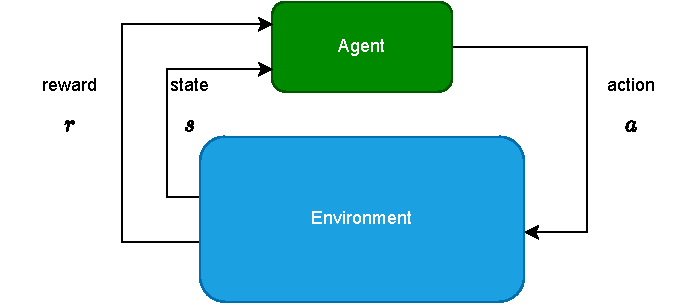
\includegraphics[width=0.5\textwidth]{images/presentation/RL_env.pdf}
    \caption{Todo}
    \label{fig:RL_env}
\end{figure}
Further, the environment is commonly described by a Markov Decision Process which is given by the tuple
$\{S, A, T, R, p(s_0), \gamma\}$ where $S$ is the set of states, $A$ the set of actions, $T: S\times A\to p(S)$ a transition
function, $R$ a reward function, $p(s_0)$ is the distribution for the initial state and
$\gamma$ is the discount factor~\cite{Moerland2020}.
Based on this, we define the policy as a function $\pi: S\times A \to p(S)$ and introduce the expected discounted reward~\cite{Schulman2015TrustRP}
\begin{equation}
    \eta(\pi) = \mathbb{E}\left[ \sum_{t=0}^\infty \gamma^t r(s_t) \right]
\end{equation}
where $s_0\sim p(s_0)$, $a_t\sim\pi(a_t|s_t)$ and $s_{t+1} \sim P(s_{t+1} | s_t, a_t)$.
Further, the state-action value function, value function and advantage function respectively are defined as
\begin{align}
    Q_\pi(s_t, a_t) &= \mathbb{E}\left[ \sum_{k=0}^\infty \gamma^kr(s_{t+k}) \right]\\
    V_{\pi}(s_t) &= \mathbb{E}\left[ \sum_{k=0}^\infty \gamma^k r(s_{t+k})  \right]\\
    A_{\pi}(s, a) &= Q_{\pi}(s,a) - V_{\pi}(s)
    \label{eq:advantage_fc}
\end{align}
where $a_t$ and $s_{t+1}$ are sampled from the respective distributions~\cite{Schulman2015TrustRP}.
%todo: fehlt hier noch etwas?
There are many possible ways to learn in the above shown framework.
Trust Region Policy Optimization and Proximal Policy Optimization both based on Policy Gradient methods which is why
will only discuss those in the following.
Now consider a policy $\pi_\theta$ which is parameterized by a set of parameters $\theta$ which must be differentiable w.r.t. the parameters~\cite{Sutton1999}.
The basic premise of policy gradient methods is to compute an estimate of the policy gradient and use it to perform gradient ascent
optimization.
One such estimator is given by
\begin{equation}
    \Hat{g} = \mathbb{E}\left[ \nabla_\theta \log(\pi_\theta(a_t | s_t)) \Hat{A}_t\right]
\end{equation}
where $\nabla_\theta$ denotes the gradient w.r.t. the parameters and $\Hat{A}_t$ the estimate of the advantage function~\cite{schulman2017ppo}.

\section{Trust Region Policy Optimization}\label{sec:trust-region-policy-optimization}
Trust Region Policy Optimization plays a vital role in understanding the Proximal Policy Optimization algorithm.
Based on the framework introduced in Section~\ref{sec:reinforcement-learning-basics} a monotonic improvement guarantee can be formulated.
One of the main contributions is the proof that such a monotonic improvement guarantee can be obtained not just for mixture policies but
also general stochastic policies which includes neural networks~\cite{Schulman2015TrustRP}.
This leads to the following theorem~\cite{Schulman2015TrustRP}:
Let $\alpha=\max_s\left \{ \frac{1}{2} \sum_i |\pi(\cdot|s)_i - \Tilde{\pi}(\cdot|s)_i| \right\}$ be the total variation divergence between
the old and the new policy.
Then the following bound holds
\begin{equation}
    \eta(\Tilde{\pi}) \geq L_{\pi}(\Tilde{\pi}) - \frac{4\varepsilon\gamma}{(1-\gamma)^2}\alpha^2
\end{equation}
where $\pi$ is the new policy, $\Tilde{\pi}$ the old policy, $\gamma$ the discount factor,
$\varepsilon = \max_{s,a} \left\{ |A_\pi(s,a)| \right\}$ and $L(\cdot)$ is a local approximation of the
discounted reward $\eta$ given by
\begin{equation}
    L_{\pi}(\Tilde{\pi}) = \eta(\pi) + \sum_s p_{\pi}(s) \sum_a \Tilde{\pi}(a|s) A_{\pi}(s, a)
\end{equation}
The same can be formulated using the Kullback-Leibler divergence instead of the total variation divergence which results in~\cite{Schulman2015TrustRP}
\begin{equation}
    \eta(\Tilde{\pi}) \geq L_{\pi}(\Tilde{\pi}) - C D_{KL}^{max}(\pi, \Tilde{\pi})
\end{equation}
where $C = \frac{4\varepsilon\gamma}{(1-\gamma)^2}$.
This allows for a chain of monotonically improving policies $\pi$.
To obtain a practical algorithm two further problems must be solved.
The policy cannot be evaluated at every state $s$ which is why the optimization problem is posed as follows
\begin{equation}
    \max_{\Tilde{\theta}} L_{\pi_{\theta}}(\pi_{\Tilde{\theta}})
\end{equation}
subject to $\mathbb{E}\left[ D_{KL}(\pi_\theta || \pi_{\Tilde{\theta}}) \right] \leq \delta$.
Here $\delta$ controls the maximum update step size of the policy.
Lastly, the formulation of the optimization problem must be converted to sampled-based estimation of the
objective function and the constraint of the optimization problem.
A practical formulation of the Trust Region Policy Optimization algorithm is shown in Algorithm~\ref{alg:trpo}
\begin{algorithm}
\caption{Trust Region Policy Optimization - Practical Algorithm}
    \begin{algorithmic}
        \Require  Hyperparameter $N, T, \dots$

        \While{termination criterion not met}
        \For{actor=$1,\dots,N$}
            \State Collect rollout buffer for $T$ steps
            \State Compute Monte-Carlo estimates of Q-values
        \EndFor
        \State Compute sample-based expectations of the objective and constraint
        \State Solve constrained optimization (conjugate gradients and line search)
        \EndWhile
    \end{algorithmic}
    \label{alg:trpo}
\end{algorithm}
Note that the conjugate gradients procedure requires second derivatives which are computationally expensive to obtain.

\section{Proximal Policy Optimization}\label{sec:proximal-policy-optimization}
The fundamental goal of the Proximal Policy Algorithm is to preserve the advantages of TRPO while using simple first-order
optimization methods which results in a simple and more efficient implementation~\cite{schulman2017ppo}.
PPO builds on the previously introduced policy gradient methods and TRPO by introducing the concept of a surrogate function
which is optimized instead.
The surrogate objective I used in the implementation and that achieved the best results is the clipped surrogate objective
which is given by
\begin{equation}
    L_{CPI}(\theta) = \Hat{\mathbb{E}}_t \left[ \frac{\pi_\theta(a_t | s_t)}{\pi_{\theta_{old}}(a_t | s_t)}\cdot \Hat{A}_t \right] = \Hat{\mathbb{E}}\left[ r_t(\theta)\Hat{A}_t \right]
\end{equation}
where $\Hat{A}_t$ is the advantage function estimate.
This is however missing the in TRPO introduced limit for the policy update which leads to excessively
large policy updates~\cite{schulman2017ppo}.
Thus, the clipped function is given by
\begin{equation}
    L_{CLIP}(\theta) = \Hat{\mathbb{E}}\left[ \min\left\{ r_t(\theta)\Hat{A}_t, \operatorname{clip}(r_t(\theta), 1-\varepsilon, 1+\varepsilon) \Hat{A}_t \right\} \right]
\end{equation}
where $\varepsilon$ is a hyperparameter controlling the largest possible policy update.
A common trick during implementation is to normalize the advantage function estimate to zero-mean and unit-variance to
increase stability during training.
A second proposed surrogate function is the adaptive KL penalty coefficient surrogate function which is given by
\begin{equation}
    L_{KLPEN}(\theta) = \Hat{\mathbb{E}}\left[ \frac{\pi_\theta(a_t | s_t)}{\pi_{\theta_{old}}(a_t | s_t)}\cdot \Hat{A}_t - \beta D_{KL}(\pi_{\theta_{old}} || \pi_\theta) \right]
\end{equation}
where the penalty coefficient $\beta$ is either halfed or doubled based on a target KL-Divergence hyperparameter~\cite{schulman2017ppo}.
The Proximal Policy Algorithm in the Actor-Critic implementation is shown in Algorithm~\ref{alg:ppo}~\cite{schulman2017ppo}
\begin{algorithm}
\caption{Proximal Policy Optimization - Actor-Critic implementation}\label{alg:ppo}
    \begin{algorithmic}
        \Require  Hyperparameter $\varepsilon, N, T, K, \dots$
        \While{termination criterion not met}
        \For{actor=$1,\dots,N$}
            \State Collect rollout buffer using current policy $\pi_{\theta_{old}}$ for $T$ steps
            \State Compute advantage function estimate $\Hat{A}_1, \dots, \Hat{A}_T$
        \EndFor
        \For{epoch=$1,\dots,K$}
            \State Optimize surrogate function $L$ w.r.t. $\theta$
            \State Update policy $\theta_{old} \leftarrow \theta$
        \EndFor
        \EndWhile
    \end{algorithmic}
\end{algorithm}
The training loop is repeated until the termination criterion is met which is given by a total number of training steps.
In a first step a rollout buffer is collected which contains a list of the visited states, the actions and observed rewards.
Based on the collected rollout buffer the advantage function estimate is computed, for this the value function is evaluated,
and the advantage function is computed following Equation~\ref{eq:advantage_fc}.
In particular, the rewards-to-go are required for the estimation.
The rewards-to-go or discounted rewards are computed for each episode in the rollout buffer by iterating the rewards
in reverse order and adding the current reward to the discounted sum.
The value function and policy are both given by neural networks which are optimized for $K$ epochs.
The policy networks uses the surrogate objective function for gradient ascent.
Further, a Huber loss is employed for the optimization of the value function network.
The PPO algorithm is very flexible to different implementations regarding the modeling of the policy and value function.
For simplicity, I have decided to model both as separate neural networks but parameter sharing between the networks is possible.
This influences the computation of the surrogate / loss function.
The architecture of the policy network is shown in Figure~\ref{fig:policy_mlp}.
A simple Multi-Layer Perceptron network with three layers is used, each layer using a $\operatorname{Tanh}(\cdot)$ activation~\cite{Goodfellow-et-al-2016}.
The output of the policy network is a mean-value which is used to construct a multi-variate gaussian distribution from which an action is sampled.
Note that the covariance is initialized as a diagonal matrix as it is assumed that there exists no dependencies between
the components.
In the following the variance used to initialize the covariance matrix is referred to as $\sigma$.
The architecture is shared by the value function network sans the action sampling and instead outputs a real number.
\begin{figure}[h]
    \centering
    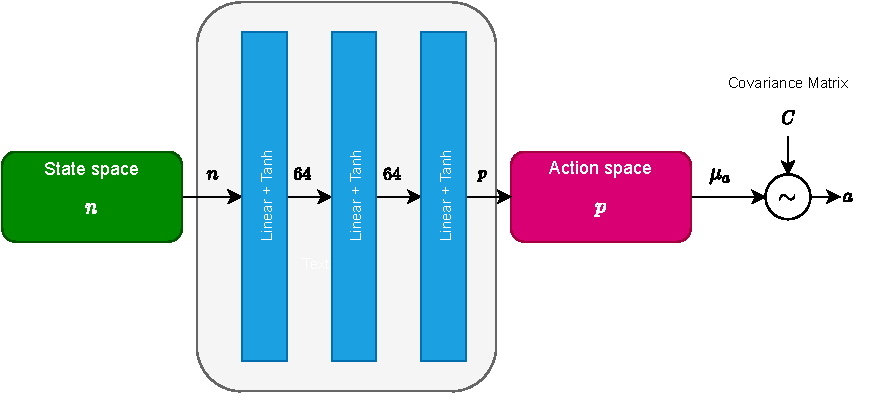
\includegraphics[width=0.7\textwidth]{images/presentation/ann_policy_value.pdf}
    \caption{Architecture of the policy MLP.}
    \label{fig:policy_mlp}
\end{figure}

\chapter{Experiments and Evaluation}\label{ch:experiments-and-evaluation}
In this chapter the experimental procedure is described in detail, and the evaluation
including the quantitative results are presented.


\section{Experimental Setup}\label{sec:experimental-setup}
I implemented the PPO algorithm in Python using PyTorch for the implementation of the
neural networks and the optimization~\cite{NEURIPS2019_9015}.
For the environments I used the openAI gym in combination with PyBulletEnv for an open-source implementation of the simulation
for the robotic environments~\cite{brockman2016openai,benelot2018}.
Further, I employed Stablebaselines3 for the normalization of the environment~\cite{stable-baselines3}.
In particular, I normalized both the state space and rewards.
The two considered environments are the Ant and Swing-up pendulum. % todo schauen welche da tatsächlich in die Auswertung kommmen
The training was conducted on an AMD Ryzen 2700X CPU for a total of X training steps. % todo: genaue Zahl einfügen
Requiring a total time of Y minutes. % todo: zeit einfügen!
The policy and value function are modeled by separate neural networks respectively.
The architecture is presented in Section~\ref{sec:proximal-policy-optimization}.
Table~\ref{tab:hyp} shows the hyperparameters.
\begin{table}[h]
    \centering
    \begin{tabular}{c|c}
        \toprule
        Hyperparameter & Value \\
        \midrule
        $\varepsilon$-clip & 0.2\\
        $\gamma$ & 0.99\\
        $\sigma$ & 0.5\\
        $N$ & 2048\\
        $T$ & 200\\
        $K$ & 10\\
        numeric stability & $1\cdot 10^{-10}$\\
        learning rate & $2\cdot 10^{-4}$\\
        \bottomrule
    \end{tabular}
    \caption{Hyperparameters used during training.}
    \label{tab:hyp}
\end{table}
The naming is in accordance with Algorithm~\ref{alg:ppo}.
Additionally, $\sigma$ refers to the variance used to initialize the covariance matrix used in the multivariate gaussian
to sample an action from the mean-value provided by the policy network.
To ensure numeric stability when normalizing the advantage function estimates the above shown hyperparameter is added
during normalization.
The learning rate is used for both the value function and policy network.

\section{Evaluation}\label{sec:evaluation}

\chapter{Discussion}\label{ch:discussion}
The primary goal of this work is to replicate the results achieved by the original PPO authors.
Thus, in Section~\ref{sec:disc_results} I discuss to what extent I was successful in reproducing the results.
In Section~\ref{sec:disc_repro}, I discuss the topic of reproducibility in science in general, and my experience in replicating the results.


\section{Results}\label{sec:disc_results}
The Pendulum-v0 environment is one of the easier environments due to its low dimensionality.
The environment is considered solved at a score of around $-140$ based on current leader boards.
Thus, to solve the environment the achieved score should either be close to $-140$ or above~\cite{Oller2020}.
The original PPO algorithm was not evaluated on this environment.
I demonstrate that the algorithm is able to solve this simple environment as my implementation was able to achieve
an average episodic return of $-175$.
This is close enough to a score of $-140$ to consider this environment solved by the algorithm.

The AntPyBulletEnv-v0 environment is significantly more complex than the Pendulum-v0 due to its higher dimensionality.
The AntPyBulletEnv-v0 was not considered in the original PPO paper.
Further, a direct comparison with the original PPO paper is difficult as they did not report absolute values but instead a score in
$[0, 1]$ where $0$ is the average episodic return of a random policy and $1$ the result of the best algorithm~\cite{schulman2017ppo}.
This comparison is of interest when comparing different algorithms to each other which is not the case in this replication study.
Thus, in the following I compare my results against the results reported in~\cite{Raffin2020}.
They reported a total average episodic return of 2160 for the PPO algorithm on the AntPyBulletEnv-v0 environment.
In comparison, the best reported algorithm, including their presented smooth exploration, is SAC gSDE and achieved a return of $3450$.
The PPO gSDE algorithm improved the vanilla algorithm to a return of $2587$~\cite{Raffin2020}.
As mentioned in Section~\ref{subsec:antpybulletenv-v0} I was unable to reproduce the results during evaluation.
However, a score around of $1250$ would be expected.
This is significantly lower than their reported return.
I identified several differences between my implementation and theirs.
Firstly, I was unable to use the same hyperparameter presented in~\cite{Raffin2020} as they lead to poor performance with
my implementation.
Due to limited resources my hyperparameters are most likely not optimal.
Further hyperparameter tuning may increase the performance by a small amount.
The original algorithm applied $\operatorname{Tanh}(\cdot)$ activations in both MLPs, I replaced them by
$\operatorname{ReLU}(\cdot)$ activations as they achieved better results in my experiments.
Lastly, my implementation of the PPO algorithm is basic and does not make use of more complex implementation details.
To name a couple of examples, I do not consider an entropy term in the loss function,
I use separate loss functions for each of the networks, and the exploration, specified by the variance in the covariance matrix,
is fixed during training.

Future work includes the implementation of the above mentioned more complex implementation details.
Apart from improving the implementation of the algorithm, many extensions have been suggested in the past years.
One such extension in regard to exploration is presented in~\cite{Raffin2020}.
Thus, the algorithm may be adapted to include current state-of-the-art approaches.


\section{Reproducibility in Science}\label{sec:disc_repro}
In science almost all work is related to previous publications either by improving established work
or comparing novel methods to the current state-of-the-art.
Thus, in order to compare your own results to the existing publications, reproducibility is extremely important.
In the context of machine learning and reinforcement learning this means that an author can validate the results of
others by running the experiments on their own machine.
However, not all authors publish their implementation which requires re-implementing their work based on the provided paper.
Many papers are relatively vague regarding implementation details and are missing vital information.
Thus, replicating results solely based on the paper is often difficult.
There are platforms helping with this problem.
One such platform is \textit{paperswithcode}\footnote{\url{https://paperswithcode.com/}}
grouping publications based on the task or dataset and offering links to available implementations.
This demonstrates some difficulties in regard to reproducibility in the field of machine learning.
Reinforcement learning introduces additional challenges as the entire framework presented in Section~\ref{sec:reinforcement-learning-basics}
is intrinsically based on statistics which further makes replicating exact results difficult.\\

In the following I would like to discuss my personal experience reproducing the results of the PPO algorithm.
Previous to this project I had no practical experience in the field of reinforcement learning except a brief introduction in a single lecture.
So the beginning included a lot of learning about the basics of reinforcement learning, common conventions and an overview of the field.
Starting with the tasks I found it relatively easy to set up an environment compatible with existing work.
Something I struggled with, especially at the beginning of the implementation, was the transfer from the formulas given in
the paper to an actual implementation, e.g.\ replacing expectations by their empirical, sample-based estimator.
The PPO paper is vague regarding the modeling of the policy and value function.
The original paper suggests the actor-critic method, it is however unclear if it is implemented as separate networks
or with parameter sharing.
Available implementations also vary widely in this point.
Once I had a working implementation, I identified some problems with hyperparameters.
To achieve optimal performance I tried to use the same hyperparameters as available implementations but depending on the
implementation they change the name of the parameters and also their definition.
This makes it difficult to copy the hyperparameters without being familiar with the respective implementation.\\
Even though I had no previous experience with reinforcement learning, I have some experience in Deep Learning
regarding reproducibility from my bachelor thesis and various projects at Team Spatzenhirn.
For me, it was significantly more difficult reproducing the results of the PPO algorithm compared to previous projects
I worked on, e.g. monocular depth estimation or object detection.
Something I noticed is that especially when transferring to a new dataset / environment the reinforcement learning
models are incredibly sensitive w.r.t.\ their hyperparameters.
I imagine that this makes it difficult to transfer a model from one of the popular dataset to an actual application.

\chapter{Conclusion}\label{ch:conclusion}
The goal of the project Deep Reinforcement Learning was to familiarize ourselves with the field of reinforcement learning,
investigate one algorithm in detail and replicate the results on a specific environment.
The contribution of this work is the implementation of a working Proximal Policy Optimization algorithm as was
demonstrated on the simple Pendulum-v0 environment and to some extent on the more complex AntPyBulletEnv-v0 environment.
Multiple reasons were identified why the implementation does not achieve the same results reported in~\cite{Raffin2020}.
Nevertheless, the implementation demonstrated the expected learning behaviour of the agent.
To further improve the performance of the algorithm current state-of-the-art approaches may be incorporated into the
standard Proximal Policy algorithm.
Lastly, reproducibility in regard to this replication study and science and general was discussed.
%\chapter{Einleitung}

Diese kleine Einleitung soll dem Nutzer helfen selbst die eigene Arbeit mit \LaTeX{} zu schreiben. Sie enth"alt Beispiele zu den wichtigsten Themen .

\blindtext

\section{Dokumentlgiederung}

Für diese Arbeit verwendet man folgende LaTeX-Kommados zur Strukturierung:

\begin{verbatim}
\chapter{Einleitung}
\section{Dokumentgliederung}
\subsection{}
\subsubsection{}
\end{verbatim}

Allerdings sollte man sich überlegen, ob man wirklich bis zur Stufe \verb|subsubsection| "Uberschriften benötigt.

\section{Illustrationen}

\blindtext

\blindtext

\subsection{Bilder und Abbildungen}

Auch in einer wissenschaftlichen Arbeit können Bilder und Abbildungen zur Veranschaulichung und zur Illustration sachlicher Inhalte integriert und einfügt werden. Für Fotografien und Bilder unterstützt PDF-\LaTeX{} direkt \verb|jpg| und \verb|png|. Ansonsten empfiehlt es sich, Vektorgrafiken zu verwenden und diese als \verb|pdf| zu speichern. Sollte ein Bild einmal von zu viel weißem Raum umgeben sein, kann man mit dem Werkzeug \verb|pdfcrop| das Bild automatisch zuschneiden.

\begin{figure}[ht]
\centering
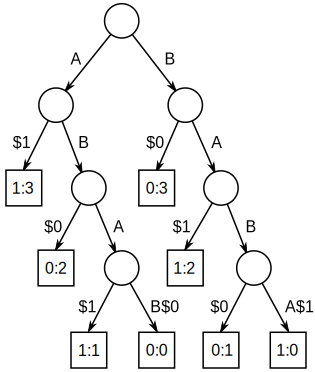
\includegraphics[width=.4\textwidth]{images/Suffix_tree_ABAB_BABA}
\caption{\label{fig:bild1}Beschreibung/Beschriftung des Bilds}
\end{figure}

Mit Hilfe eines Labels \verb|\label{fig:bild1}| kann man sich dann im fortlaufenden Text mittels eines Querverweises auf diese Grafik beziehen: \verb|\ref{fig:bild1}|. An der Stelle des ref-Kommandos platziert LaTeX die Nummer der Abbildung: \glq siehe Abbildung \ref{fig:bild1}\grq.


\subsection{Tabellen}
\label{sec:tabellen}

Seite \pageref{tab:beispieltabelle}, Abschnitt \ref{sec:tabellen}, enthält Beispieltabelle \ref{tab:beispieltabelle}. In vielen \LaTeX{}-Büchern finden sich gute Anleitungen zum Erstellen von Tabellen. Komplexere Tabellen können sinnvollerweise in Excel oder einer anderen Tabellenkalulation vorgefertigt und mit einem Umwandlungsprogramm oder -werkzeug in LaTeX-Quellcode konvertiert werden.

\begin{table}[h]
\begin{center}
\begin{tabular}{|lll|}
    \hline
	A & B & C \\
	\hline
	x & x & x \\
	x & x & x \\
	\hline
\end{tabular}
\end{center}
\caption{Eine kleine Beispieltabelle}
\label{tab:beispieltabelle}
\end{table}


\subsection{Formeln}

Mathematische Formeln lassen sich in der Umgebung  \verb|math| erzeugen. Die Kurz- Schreibweise lautet \verb|\( a^2+b^2=c^2 \)|;  hierbei steht die Formel dann im laufenden Text: \( a^2+b^2=c^2 \). Die kürzeste Form ist mit zwei \verb|$| um die Formel, z.B.~so: Wasser ist H$_2$O. \verb|H$_2$O|

Mit der Schreibweise \verb|\[ y=x^2 \]| wird die Formel mittig in einer eigenen Zeile gesetzt, z.B.

\[y = x^2 \]

Formeln in der Umgebung \verb|equation| werden mittig in einer eigenen Zeile gesetzt und fortlaufend nummeriert:

\begin{equation}
x_{1,2} = \frac{-b\pm\sqrt{b^2-4ac}}{2a}
\label{mitternachtsformel}
\end{equation}
Wenn wir z.B.~über die beliebte Mitternachtsformel (Gleichung \ref{mitternachtsformel}) Details im umliegenden Text schreiben wollen, lässt sich diese wie ein Bild oder eine Tabelle referenzieren, sofern man ihr ein Label zugewiesen hat..


\subsection{Programmier-Code}

Mehrzeiliger Programmier- und Quellcode kann mit \verb|verbatim| in einer Umgebung gesetzt werden:

\begin{verbatim}
  Dieser Text steht in einer verbatim-Umgebung und wird daher
  in Schreibmaschinenschrift geschrieben.
  LaTeX-Kommandos, z.B. \includegraphics[width=.6\textwidth]{bild.jpg}
  werden nicht interpretiert, sondern "verbatim" ausgegeben.
\end{verbatim}

Schöner und professioneller lässt sich Programmier-Code mit dem \verb|listings|-Paket, eingeben, formatieren und ausgeben. Dazu kann man in der Präambel die Sprache angeben, in der die Quellcodes geschrieben sind.

\begin{lstlisting}
public class Hello {
    public static void main(String[] args) {
        System.out.println("Hello World");
    }
}
\end{lstlisting}

Innerhalb einer Zeile gibt man Wörter am Besten als \verb|\verb##| an, dabei erwartet \LaTeX{} zweimal das gleiche Zeichen als Begrenzer. Im Beispiel ist dies die Raute \verb|#|, man kann aber auch jedes andere Zeichen nehmen, z.B. das Plus $+$.



\section{Text}

Textteile können bei Bedarf mit dem Befehl \verb|\emph{}| \emph{hervorgehoben} werden. Falls in einem Satz ein Punkt vorkommt, macht man danach kein Leerzeichen sondern eine Tilde (\verb|z.~B.~so!|), denn dann fügt \LaTeX{} den korrekten Abstand ein, z.~B.~so!


In der Präambel der vorliegenden tex-Datei gibt es den Befehl \verb|hypenation|, der zur Silbentrennung da ist. \LaTeX{} verfügt zwar über  eine eingebaute Silbentrennung, die jedoch bei manchen Wörtern falsch trennt. Damit diese Wörter korrekt getrennt werden, gibt man sie dann mit dem Befehl in der Präambel an\footnote{Das Wort \emph{Silbentrennung} ist hier das Beispiel}.

Fußnoten werden mit dem Befehl \verb|footnote| mitten in den fortlaufenden Text eingefügt. \footnote{Wie man schon im vorherigen Absatz sehen konnte.}

In wissenschaftlichen Arbeiten muss man des öfteren andere Arbeiten zitieren. Dazu nutzt man die Stiloptionen und Zitierbefehle des Pakets \verb+biblatex+, z.\,B.\,\verb|numeric| (=Standard-Stil) oder \verb|verbose| resp. \verb|\cite{name}| oder \verb|\autocite{name}|. In eckigen Klammern kann man noch die Seitenzahl angeben, falls notwendig. Der Name ist ein Schlüssel aus der Datei \verb|bibliography.bib|. Falls einmal ein Werk nur indirekt zu einem Teil der Arbeit beigetragen hat, kann man es auch mit \verb|nocite| angeben, dann landet es in der Literaturliste, ohne dass es im Text ausdrücklich zitert wird.


\subsection{Weiterführendes}

Zum Schluss sei auf die Vielzahl an Büchern zu \LaTeX{} verwiesen. In jeder Bibliothek wird sich eine Einführung finden, in der dann weitere Themen wie mathematische Formeln, Aufbau von Briefen und viele nützliche Erweiterungen besprochen werden.


% hier weitere Kapitel einbinden

\appendix
% hier Anhänge einbinden

\backmatter
\nocite{Knappen2009}
\nocite{Mittelbach2005}
\nocite{Schlosser2014}
\nocite{Sturm2012}
\nocite{Voss2010}

\printbibliography

\clearpage
\thispagestyle{empty}

Name: \fullname \hfill Matrikelnummer: \matnr \vspace{2cm}

\minisec{Erklärung}

Ich erkläre, dass ich die Arbeit selbständig verfasst und keine anderen als die angegebenen Quellen und Hilfsmittel verwendet habe.\vspace{2cm}

Ulm, den \dotfill

\hspace{10cm} {\footnotesize \fullname}
\end{document}
